\chapter{Simulations of the Bornholdt model}\label{ch:chapter3}
\section{Results}
We performed a numerical simulation of the Bornholdt model, with 1024 spins arranged on a square lattice. The values for the parameters are: $J=1.0$, $\alpha=4.0$, $T=1/\beta=1.5$. 
\subsection{Dynamics of the strategies}
The simulations have shown that the initial distribution of the agent's strategy is irrelevant, as the system quickly converges to a state where between 50\% and 70\% of the agents follow the strategy $C_i(t) = 1$, as can be seen from figure \ref{fig:strategies}.

\begin{figure}[H]
    \centering
    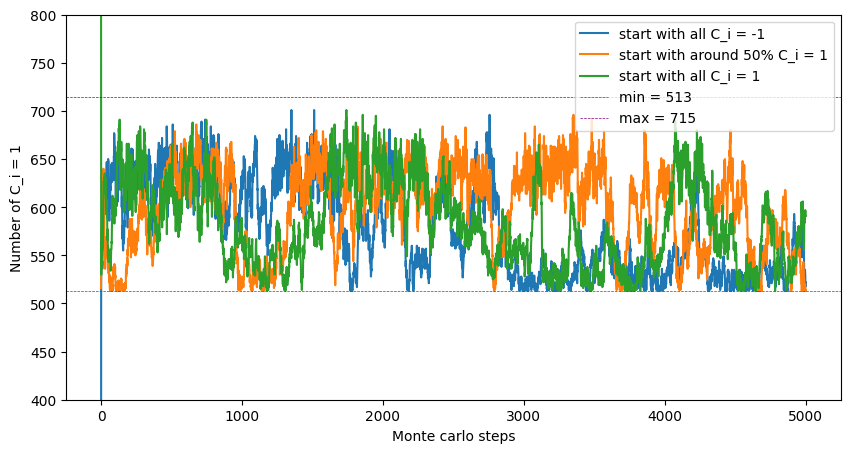
\includegraphics[width=1\textwidth]{c_values.png}
    \caption{Dynamics of agent's strategy based on different starting distributions.}
    \label{fig:strategies}
\end{figure}

\subsection{Dynamics of the price}
We can see the dynamics of the price (i.e. the magnetization) in figure \ref{fig:magnetization}.

By looking at the spin configurations at different times (figure \ref{fig:lattices}), we can see that the system alternates between metastable and turbulent states.

\begin{figure}[H]
    \centering
    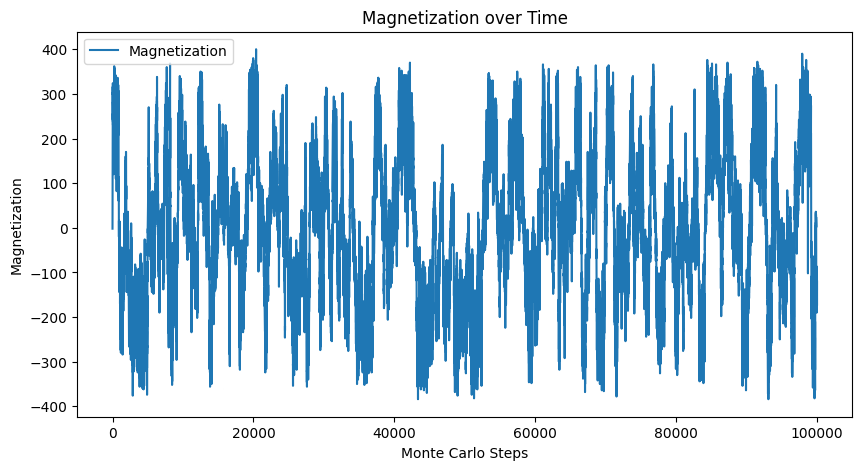
\includegraphics[width=1\textwidth]{magnetization.png}
    \caption{Dynamics of the magnetization of the system.}
    \label{fig:magnetization}
\end{figure}

\begin{figure}[H]
    \centering
    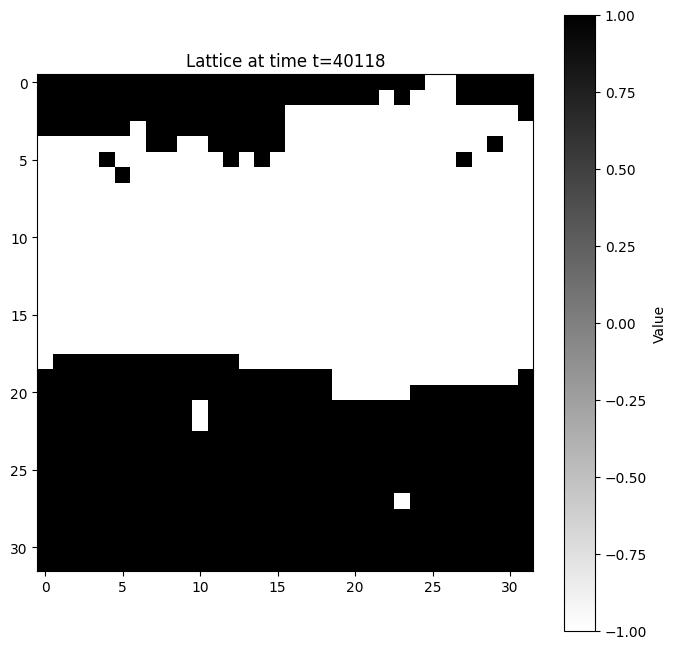
\includegraphics[width=0.3\textwidth]{40118.png}
    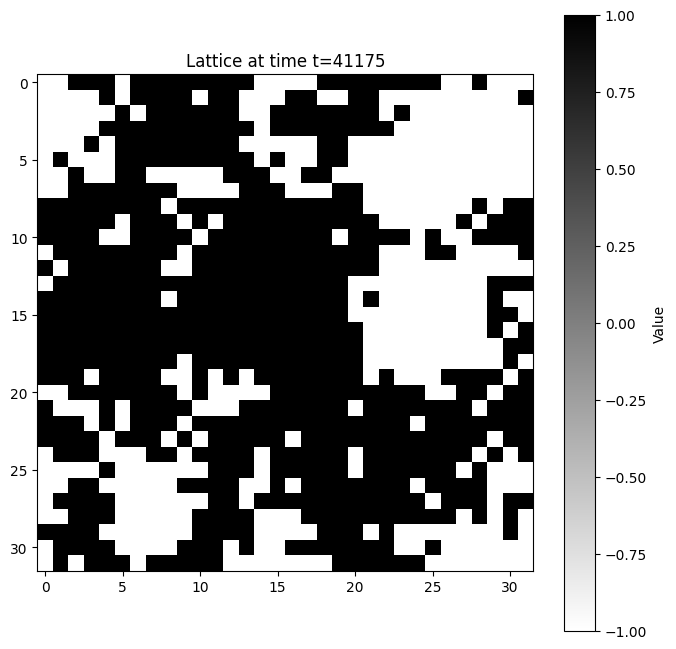
\includegraphics[width=0.3\textwidth]{41175.png}
    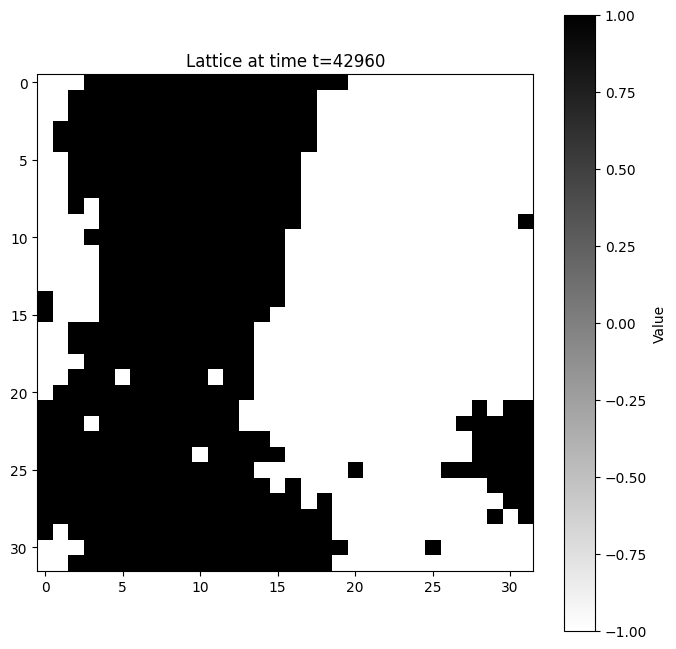
\includegraphics[width=0.3\textwidth]{42960.png}
    \caption{Snapshots of the lattices at times $t=40118$, $t=41175$ and $t=42960$.}
    \label{fig:lattices}
\end{figure}

\subsection{Dynamics and statistical properties of the returns}
By interpreting the magnetization as the price of the financial asset, we can calculate the log-returns of the asset as $\log(M(t)/M(t-1))$. Actually, to make sure the returns are well-defined, we use the absolute value of the magnetization, $|M(t)|$. The time-series of the returns is shown in figure \ref{fig:returns}.

\begin{figure}[H]
    \centering
    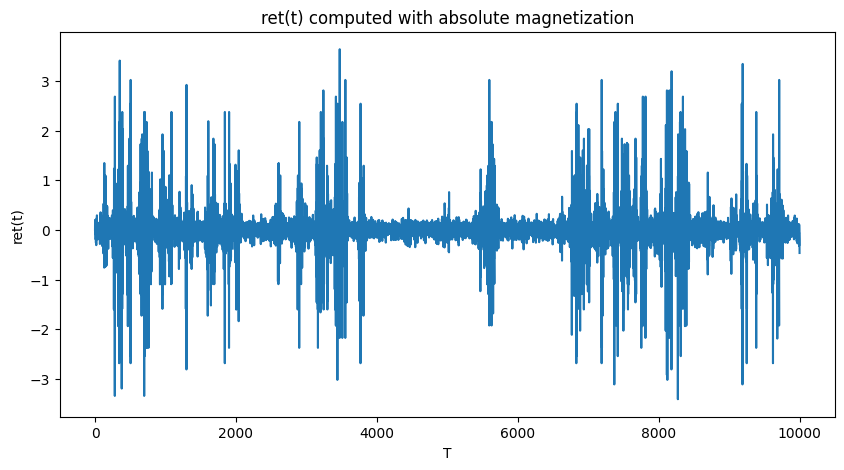
\includegraphics[width=1\textwidth]{returns.png}
    \caption{Time-series of the returns of the asset.}
    \label{fig:returns}
\end{figure}

From a financial perspective, we are interested in checking wether the returns exhibit the statistical properties of real financial data, namely fat tails and autocorrelation, as noted in \cite{bouchaud2000theory}.

\subsubsection{Fat tails}
A plot of the distribution of the returns, as shown in figures \ref{fig:returns_distribution} and \ref{fig:cumulative_returns_distribution}, indicates that the returns indeed seem fat-tailed. A QQ-plot of the returns against a normal distribution (figure \ref{fig:qqplot}) confirms this.

\begin{figure}[H]
    \centering
    \begin{minipage}{0.48\textwidth}
        \centering
        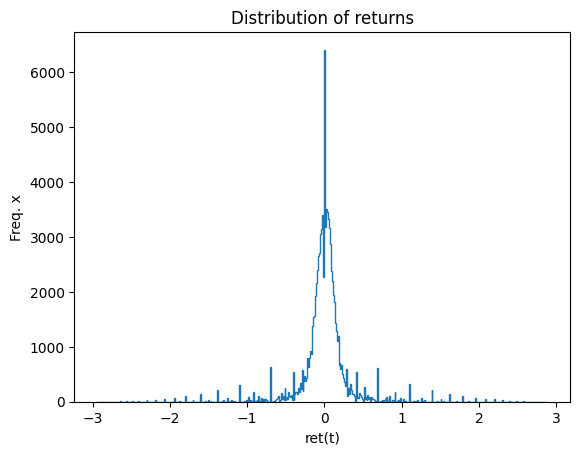
\includegraphics[width=\textwidth]{distribution_returns.png}
        \caption{Distribution of the returns of the asset.}
        \label{fig:returns_distribution}
    \end{minipage}
    \hfill
    \begin{minipage}{0.48\textwidth}
        \centering
        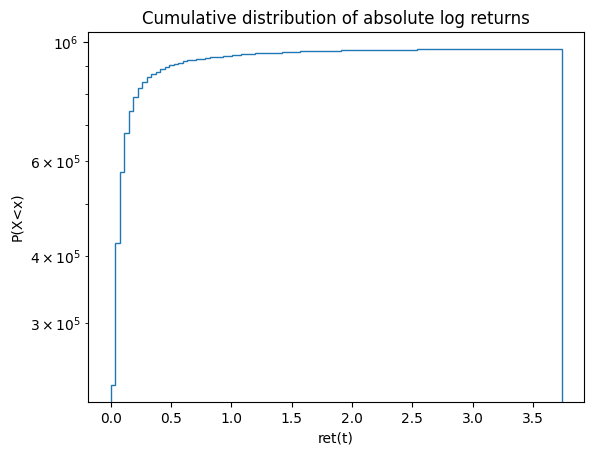
\includegraphics[width=\textwidth]{cumulative_distribution.png}
        \caption{Cumulative distribution of the returns of the asset.}
        \label{fig:cumulative_returns_distribution}
    \end{minipage}
\end{figure}


\begin{figure}[H]
    \centering
    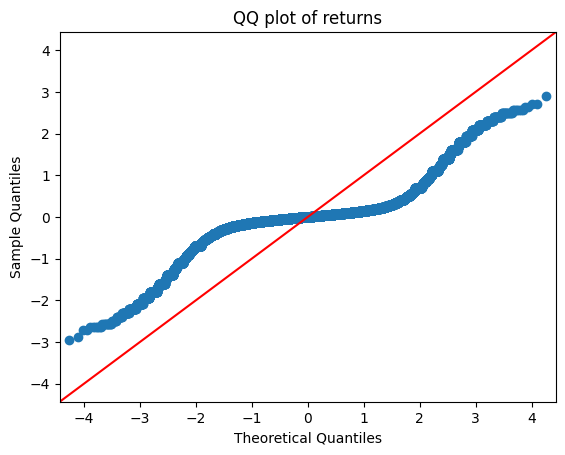
\includegraphics[width=0.5\textwidth]{qqplot-returns.png}
    \caption{QQ-plot of the returns against a normal distribution.}
    \label{fig:qqplot}
\end{figure}

\subsubsection{Autocorrelation}
The autocorrelation function of the returns is shown in figure \ref{fig:autocorrelation}. We can see that the autocorrelation is significant for a large number of lags, which is consistent with the empirical observation that financial returns are autocorrelated.

\begin{figure}[H]
    \centering
    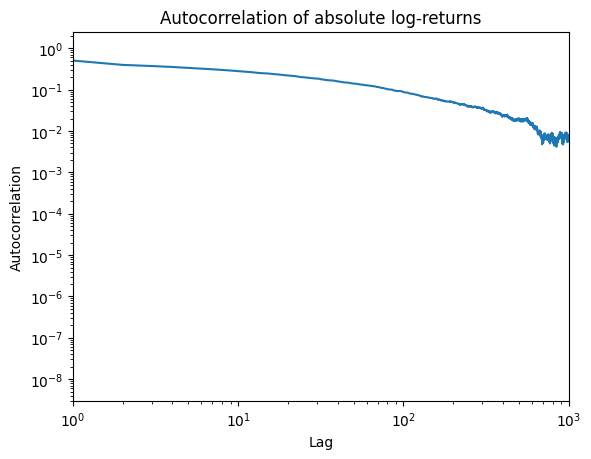
\includegraphics[width=0.5\textwidth]{autocorrelation.png}
    \caption{Autocorrelation function of the returns.}
    \label{fig:autocorrelation}
\end{figure}

\section{Financial implications}
The results of the simulation suggest that the Bornholdt model is able to reproduce some of the statistical properties of real financial data, such as fat tails and autocorrelation of returns. This is interesting because the model is based on a simple spin model, and does not rely on any assumptions about the rationality of agents or the efficiency of markets.

The model also suggests that the dynamics of the price are driven by the interaction between agents, rather than by external factors such as news or economic indicators. This is consistent with the idea that financial markets are complex systems, where the interactions between agents can lead to the emergence of collective behaviour.

The key assumptions of models such as \cite{black_scholes} are that the price of the underlying asset follows a geometric Brownian motion, and that the agents in the market are rational and risk-neutral. The Bornholdt model challenges these assumptions by showing that the price dynamics can be driven by the interaction between agents, and that the returns can exhibit fat tails and autocorrelation.